\documentclass[tikz,margin=10pt]{standalone}
\usepackage[utf8]{inputenc}
\usepackage[T1]{fontenc}

\usepackage{tikz}
\usepackage{helvet}
\usepackage{amsmath}
\usepackage{circuitikz}

\renewcommand\familydefault\sfdefault

\usetikzlibrary{calc}

\definecolor{baseColor}{RGB}{18, 54, 69}
\definecolor{accentColor}{RGB}{1, 103, 143}
\definecolor{complementColor}{RGB}{254, 152, 112}

\begin{document}
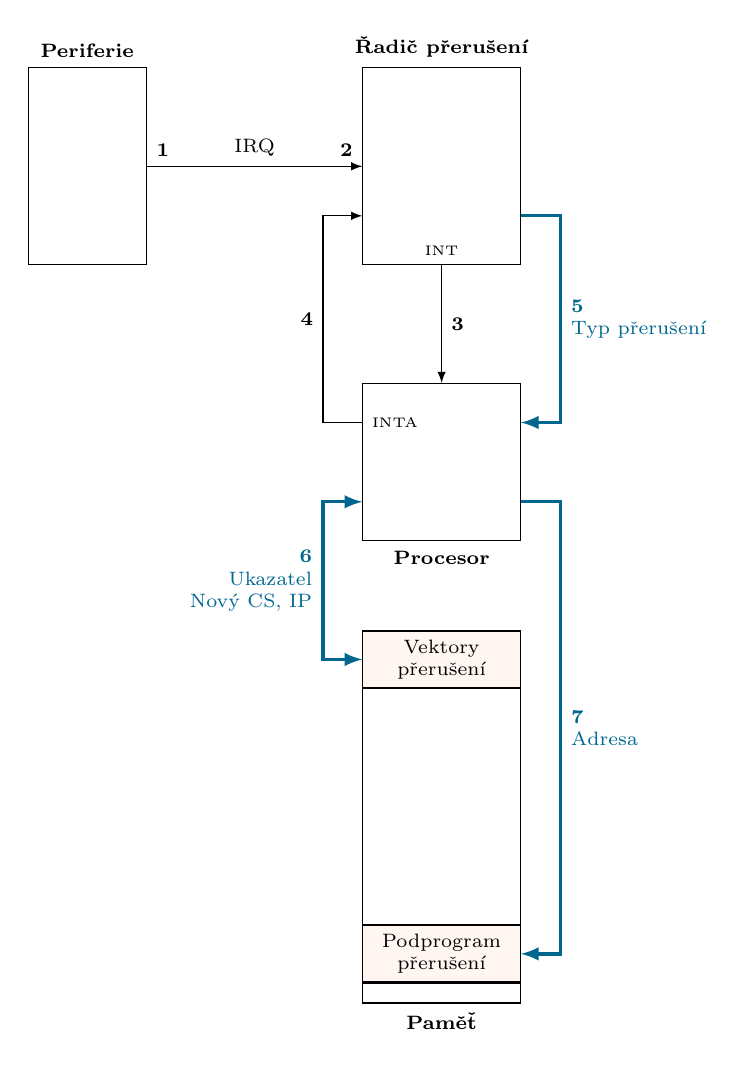
\begin{tikzpicture}[
    every node/.style={font=\scriptsize},
    inner memory/.style={draw, inner sep=3pt, minimum width=2cm, align=center},
    inner memory highlight/.style={inner memory, font=\scriptsize, fill=complementColor!10!white},
    arrow label/.style={midway},
    left arrow label/.style={arrow label, left, align=right},
    right arrow label/.style={arrow label, right, align=left},
    chip/.style={anchor=south, draw, inner sep=0pt, minimum width=2cm, minimum height=2.5cm}
]

    \node [matrix, draw, inner sep=0pt] (mem) at (0,0) {
        \draw node[inner memory highlight] (int_vec) {Vektory\\přerušení};    \\
        \draw node[inner memory, minimum height=3cm] {};                      \\
        \draw node[inner memory highlight] (int_isr) {Podprogram\\přerušení}; \\
        \draw node[inner memory, minimum height=.25cm] {};                    \\
    };
    \draw (mem.south) node[below] {$ \text{\textbf{Paměť}} $};

    \draw (mem) ++(0, 3.5) node[chip, minimum height=2cm] (cpu)  {};
    \draw (cpu.south) node[below] {$ \text{\textbf{Procesor}} $};

    \draw (cpu) ++(0, 2.5) node[chip] (pic)  {};
    \draw (pic.north) node[above] {$ \text{\textbf{Řadič přerušení}} $};

    \draw (pic) ++(-4.5, 0) node[chip, anchor=center, minimum width=1.5cm] (io) {};
    \draw (io.north) node[above] {$ \text{\textbf{Periferie}} $};

    \draw[-latex, accentColor, very thick] 
        ($ (cpu.north east)!.75!(cpu.south east) $) 
     -- ($ (cpu.north east)!.75!(cpu.south east) +(.5, 0) $) 
     to node[right arrow label] {\textbf{7}\\Adresa}(\tikztostart|-int_isr.east) 
     -- (int_isr.east);
 
    \draw[latex-latex, accentColor, very thick] 
        ($ (cpu.north west)!.75!(cpu.south west) $) 
     -- ($ (cpu.north west)!.75!(cpu.south west) -(.5, 0) $) 
     to node[left arrow label] {\textbf{6}\\Ukazatel\\Nový CS, IP} (\tikztostart|-int_vec.west) 
     -- (int_vec.west);

    \coordinate (cpu_inta) at ($ (cpu.north west)!.25!(cpu.south west) $);
    \draw[latex-] 
        ($ (pic.north west)!.75!(pic.south west) $) 
     -- ($ (pic.north west)!.75!(pic.south west) -(.5, 0) $) 
     to node[left arrow label] {\textbf{4}}(\tikztostart|-cpu_inta) 
     -- (cpu_inta);
     \draw (cpu_inta) node[right] {$ \text{\tiny INTA} $};


    \coordinate (cpu_irq_type) at ($ (cpu.north east)!.25!(cpu.south east) $);
    \draw[-latex, accentColor, very thick] 
        ($ (pic.north east)!.75!(pic.south east) $) 
     -- ($ (pic.north east)!.75!(pic.south east) +(.5, 0) $) 
     to node[right arrow label] {\textbf{5}\\Typ přerušení} (\tikztostart|-cpu_irq_type) 
     -- (cpu_irq_type);

    \draw (pic.south) node[above] {$ \text{\tiny INT} $};
    \draw[-latex] (pic.south) -- (cpu.north) node[right arrow label] {\textbf{3}};

    \draw[-latex] (io.east) -- (pic.west) node[left arrow label, above] {IRQ};
    \draw (io.east) node [above right] {\textbf{1}};
    \draw (pic.west) node [above left] {\textbf{2}};
\end{tikzpicture}
\end{document}